\section{Building the fine-only baseline}
\label{sec:supp_baseline}
The hierarchy of the main paper replaces the propagation of an earlier, fully registered pipeline: CA seed $\rightarrow$ one 64-pixel SA module, two observation-wise passes $\rightarrow$ DenseCRF, with SA restricted to calls 10--20. This section records how that baseline was selected; it is the ``fine only'' reference throughout the main paper.

\paragraph{One SA module.}
One pass through all sixteen SA modules improves the frozen seed, but the last 64-pixel module (\texttt{up\_blocks.3.attentions.2}) is better. OOF mIoU rises from 0.756 to 0.789 in the combined SA confirmation, all five folds select it, and the paired mean-image gain is $+0.042$ (CI $[+0.037,+0.047]$). Separate screens favoured call 30, resolutions 8+64 and heads $\{1,4,6\}$, but none survived the combination. A Cartesian audit of six CA seeds and twelve SA settings found module 15 the best SA partner for every seed.

\paragraph{Two observation-wise passes.}
For each call--head observation $i$, the fine-only map is
\begin{equation}
p_2=\frac1{|\mathcal I|}\sum_{i\in\mathcal I}A_i^2c .
\end{equation}
The square is taken within each observation before averaging, which is a different operator from $(\frac1{|\mathcal I|}\sum_iA_i)^2c$. A second pass raises OOF mIoU from 0.788 to 0.800, especially for chair ($+0.078$) and person ($+0.030$); a third pass is not promoted. Figure~\ref{fig:supp_depth} shows the trade-off between completion and leakage. In a later diagnostic (A3 seed, calls 10--20, threshold 0.425), pixels first accepted at depth one are 86.5\% true positives on VOC-Sim and 70.8\% on COCO-Cap, but pixels first accepted at depth three are only 39.3\% and 14.0\%.

\begin{figure*}[t]
\centering
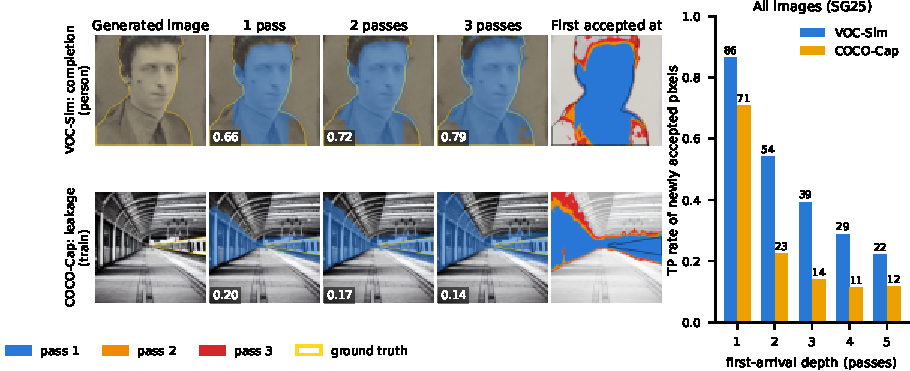
\includegraphics[width=\textwidth]{figures/propagation_depth.pdf}
\caption{\textbf{How far fine SA should propagate.} Left: one, two and three observation-wise passes on a completion example (VOC-Sim, 90th percentile of the two-pass gain) and a leakage example (COCO-Cap, 10th percentile of the three-pass gain), with the pass at which each pixel was first accepted. Right: true-positive rate of newly accepted pixels by depth, pooled over all images. The supplementary gallery (Fig.~\ref{fig:supp_propagation_depth}) applies both rules to both datasets.}
\label{fig:supp_depth}
\end{figure*}

\paragraph{Refinement absorbs propagation gains.}
DenseCRF was selected in all five folds and improved all 20 classes in its screen (0.788$\rightarrow$0.805); with two passes the combined system reached 0.813 OOF. Twenty-four families of graph operators were then registered against one pass (Sec.~\ref{sec:supp_packages}). Observation-reliability operators (consensus edges, sign consensus, robust aggregation, keeping the 50\% most consistent observations) raised one-pass mIoU to 0.797--0.798, which is the level of a second pass. Their per-class gains also correlate with those of the second pass (0.88 and 0.82), and none survived on top of two passes plus DenseCRF. Graph-restricting operators (absorbing walks, confidence locks, reciprocal links, bottlenecks, region labelling) lost. From then on, every candidate was selected on the refined mask.

\paragraph{The SA call window.}
Selecting on the refined mask found one change: SA calls 10--20 instead of 0--30 (Table~\ref{tab:supp_sg22}). Late calls recover some object pixels but also add distant false positives (Fig.~\ref{fig:supp_temporal}), and their utility varies by class.

\begin{table}[t]
\centering
\footnotesize\setlength{\tabcolsep}{3pt}
\begin{tabular}{@{}lccccc@{}}
\toprule
Setting & P2 & R2 & Mid & Forced OOF & COCO \\
\midrule
One pass & -- & -- & -- & .7873 & .6172 \\
Two passes & $\checkmark$ & -- & -- & .7997 & .6246 \\
+ DenseCRF & $\checkmark$ & $\checkmark$ & -- & .8132 & .6372 \\
+ calls 10--20 & $\checkmark$ & $\checkmark$ & $\checkmark$ & .8168 & .6438 \\
\bottomrule
\end{tabular}
\caption{\textbf{The fine-only baseline in one run} (SG22, uniform seed). The registered selector chose MID-P2+R2 in four of five folds (selection path 0.8158 OOF).}
\label{tab:supp_sg22}
\end{table}

\begin{figure*}[t]
\centering
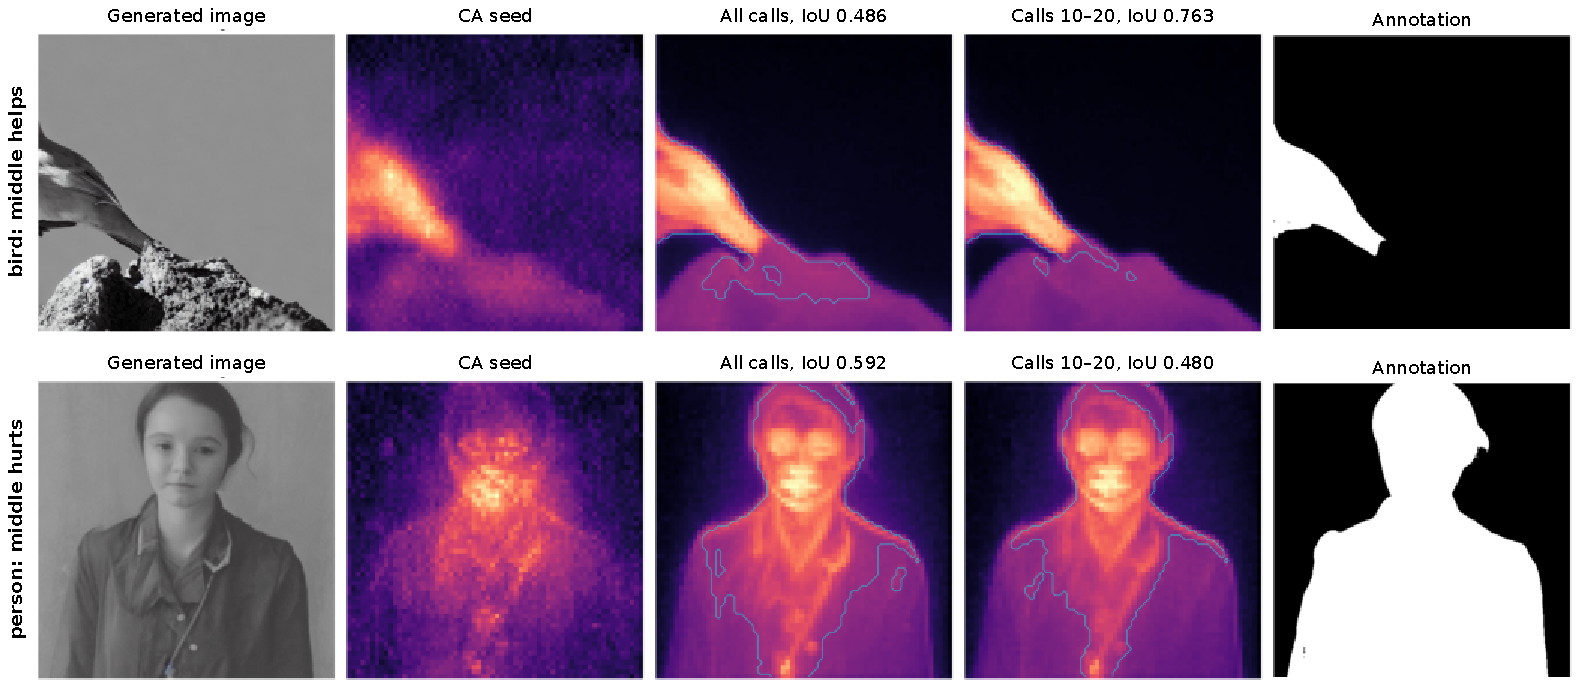
\includegraphics[width=\textwidth]{figures/temporal_tradeoff.pdf}
\caption{\textbf{A temporal window can remove leakage or remove object pixels.} Two VOC-Sim examples from the one-pass, raw-map diagnostic, propagated with SA calls 0--30 or 10--20. Bird gains when a false region is suppressed; person loses when useful extent is suppressed. These are deliberately opposing examples, not images from the final evaluation.}
\label{fig:supp_temporal}
\end{figure*}
\clearpage
